\documentclass[a4paper]{scrartcl}
\usepackage[utf8]{inputenc}
\usepackage[english]{babel}
\usepackage{graphicx}
\usepackage{lastpage}
\usepackage{pgf}
\usepackage{wrapfig}
\usepackage{fancyvrb}
\usepackage{fancyhdr}
\pagestyle{fancy}
\usepackage{dingbat}

\usepackage[autostyle]{csquotes}
\usepackage[
    backend=biber,
    style=ieee,
    sortlocale=de_DE,
    natbib=true,
    url=true,
    doi=true,
    eprint=false
]{biblatex}
\addbibresource{id1354-report-template.bib}

\usepackage[]{hyperref}
\hypersetup{
    colorlinks=true,
}

% Create header and footer
\headheight 27pt
\pagestyle{fancyplain}
\lhead{\footnotesize{Internet Applications, ID1354}}
\chead{\footnotesize{Jacobs tasty website!}}
\rhead{}
\lfoot{}
\cfoot{\thepage\ (\pageref{LastPage})}
\rfoot{}

% Create title page
\title{Jacobs tasty website!}
\subtitle{Internet Applications, ID1354}
\author{Jacob Kimblad jacobki@kth.se}
\date{2018-11-05}

\begin{document}

\maketitle

%\section*{Tips for Report Writing}
%\textbf{REMOVE THIS SECTION BEFORE SUBMITTING THE REPORT.}\\

%\noindent \textit{The target audience has exactly the same skills as the author, except they do not know anything at all about the specific program described in the report.} \\

%Consider the following:

%\begin{itemize}
%\item \textbf{The report must be \textit{centered around the requirements}. Which are they (Introduction), how did you work to meet them (Method), what is the solution that meets them (Result), and how can you be sure they are met (Discussion). This is the IMRaD method.}

%\item \textbf{The report must show that you have done the work yourself and that you have understood what you have done. Both of these goals are met by carefully explaining the source code.}

%\item Is spelling and grammar correct? Is spoken language avoided?

%\item Does the report have a good structure with sections, subsections and paragraphs?

%\item Is the solution clearly explained? Will the reader understand the program? What would you yourself want to know if you read about the program, is that included in the report?

%\item Is the solution analyzed and evaluated? Are important properties of the program explained? Should there have been more extensive evaluation?

%\item Is the text clarified with images and/or other figures, and with links to the code in your Git repository? Remember that all figures (images, tables, graphs, code listings, etc) shall be numbered and have a short explaining text.
%\end{itemize}

\section{Introduction}
The first requirement for the tasty recipes web site is that it should constist of four different pages. An index page, a calendar page, a meatballs recipe page and a pancakes recipe page. The second requirement is that from each of the four web pages you should be able to navigate to any of the other three web pages directly. The third requirement is that they should all have a similar layout which should be put into consideration when choosing fonts, colors, mouse hoovering, and link behaviour. In addition to all of the pages having similar layout some of their properites may not be assigned their default values. These properites are page layout, font family, font size, font style, foreground and background color, mouse hovering and link behavior. Beneath follows the requirements for each of the four individual pages.

\subsection{Index page}
The index page should be informative and welcoming by promoting the calendar page and providing a link to it in text-format.

\subsection{Recipe pages}
There should be an individual page for each of the two recipes (pancakes and meatballs). The recipe page should contain a picture of the prepared dish, its ingredients, instructions for preparing, its name and hard coded user comments.

\subsection{Calendar page}
The calendar page should, as the name suggests, present the user with a calendar of the month. Two days in the calendar should each contain a unique picture of the recipes (meatballs and pancakes). These should be clickable links that redirects the user to their respective recipe page.

\subsection{Tasks}
The tasks to be followed which should meet the requirements begin with creating HTML and CSS files to implement each of the different pages of the tasty recipes web site. It is necessary that all of the HTML and CSS files pass the W3C validation. It is also necessary to use a reset style sheet. When designing the website it is necessary to follow five of the ten heuristics for user interface design which were discussed during a lecture. All of the pages must also have identical behavior in the following four browsers: Chrome, Explorer (or Edge), Firefox and Safari.


\subsection{Summary}
The following bulle list summarises the requirements and functionality of the complete web page.
\begin{itemize}

    \item Design and functionality:
        \begin{enumerate}
            \item Contain index, calendar and recipe pages.
            \item Navigate to any page directly from any other page.
            \item Pages should use similar layout.
            \item Properties that must not have default values.
        \end{enumerate}

    \item Index page:
        \begin{enumerate}
            \item Informing and welcoming.
            \item Contains a link to the calendar page.
        \end{enumerate}

    \item Recipe pages:
        \begin{enumerate}
            \item One page for each recipe.
            \item Contain the name of the dish.
            \item Contain a picture of the prepared dish.
            \item Contain a list of required ingredients.
            \item Contain steps of how to prepare the dish.
            \item Contain comments from users about the dish. 
        \end{enumerate}

    \item Calendar page:
        \begin{enumerate}
            \item Present a calendar of one month.
            \item Present a picture of each recipe in two unique days.
            \item Make the pictures of the recipes clickable links to their respective page.
        \end{enumerate}

    \item Tasks:
        \begin{enumerate}
            \item Implement the described pages using CSS and HTML.
            \item All CSS and HTML files should pass W3C validations.
            \item Use a CSS reset sheet.
            \item Follow the five given heuristics for user interface design.
            \item All pages must have identical behaviour in the four common browsers.
        \end{enumerate}

\end{itemize}

%\textbf{This section tells \textit{what} are you going to do.} \\

%\noindent Explain the task and the requirements on the solution. It is very important to \textit{clearly state the requirements}. If you wrote the program together with other students, list their names and email addresses here.

\section{Literature Study}
For basic CSS and HTML syntax and tutorials reference \citet{noauthor_w3schools_nodate} provides good overview of possible syntax for both languages. It also provides easy to understand examples and the limits and possibilities of different tags in HTML and selectors, properties and values in CSS. It also provides templates for websites using HTML and CSS which is a great resource to gather inspiration and examples of actual websites.

It is predicted that the hardest part to complete will be to get the formating right for the calendar using HTML and CSS. The stackoverflow post shown in \citet{noauthor_html_nodate-1} explains how the HTML table tag should not be used to format layout of the page. It should only be used for data that is very tabular in nature. When looking at the reference document for the table tag \citet{noauthor_html_nodate} we see that a lot of table attributes have been deprecated in HTML5. Reference \citet{noauthor_using_nodate} explains how using tables for layout is now offcially wrong and instead div elements should be used. To help with constructing a layout for the calendar a div table generator such as \citet{noauthor_div_nodate} can be used.


%This section must prove that you collected sufficient knowledge before starting development, instead of just hacking away without knowing how to complete the task. State what you have read and briefly summarize what you have learned.

\section{Method}

To solve the tasks a set of development tools are selected either becuase the authors familiarity with them or because of their simplicity to use, both of which helps to speed up development time. The text editor used to edit the HTML and CSS files is Vim, described as "Vim is a highly configurable text editor for efficiently creating and changing any kind of text" \citet{noauthor_welcome_nodate}. The web server used is the http-server \citet{noauthor_http-server_nodate} acquired under the NodeJS infrastructure. The shell used to run both Vim and the http-server is Zsh \citet{noauthor_zsh_nodate} under a GNU/Linux operating system distribution known as Manjaro \citet{noauthor_manjaro_nodate}. For source control Git was used with Github hosting a remote repository, this made it such that the validation tools, described in the next paragraph, could be used by just provdiging them with the URL's to the raw files hosted on Github.

Testing tools are also used to check some of the requirements of the web site are met. To make sure that the HTML files passes a W3C validation the online testing tool found in \citet{noauthor_w3c_nodate} is used. A similar testing tool is also used for the CSS files such that they also pass a W3C validation, this testing tool can be found at \citet{noauthor_w3c_nodate-1}.

To help with debugging the code the web browser Firefox is used as it also includes a very handy set of tools, known as the Firefox Developer Tools \citet{noauthor_firefox_nodate}, that can be used to change the source code and see the effects in real time all within the browser. This helps with speeding up development time, as there is no need to navigate around different tools to make and the see the effects of a simple change. It is also necessary to test the finalised code such that it gives the exact desired behaviour in all of the different browsers defined by the requirements. To do this another online tool found at \citet{online browser tester} was used.

%\textbf{This section tells \textit{how} you solved the task.} \\

%\noindent Explain how you worked when solving the tasks and how you evaluated that your solution met the requirements. Mention development tools and IDEs you used. \textit{Do not explain your solution and do not refer to code}, that belongs to the \textit{Result} section.

\section{Result}

To make sure that every other page can be reached from any of the four pages a navigation bar at the top of each page is used. This navigation bar has the same look and layout for all four pages to fulfill the requirement of similar layout on all the pages and can be seen in figure \ref{fig:navbar}.

\begin{figure}[h!]
    \begin{center}
        
\includegraphics[scale=0.5]{images/navbar.png}
        \caption{A sample user interface screenshot to illustrate the navigation bar at the top of each page.}
        \label{fig:navbar}
    \end{center}
\end{figure}

To get the same behaviour from all different browsers a reset style sheet was used which can be found in \citet{kimblad_git_2018}. This was referenced from every single html file as to correctly reset the wanted css properties, the references can be seen at \citet{kimblad_git_2018-reset}.

To make sure all pages have a similar layout a single custom stylesheet were used for all four of the pages which defines some custom properties of the page such as the fonts used, font sizes, font colors for headings \citet{kimblad_git_2018-h1}\citet{kimblad_git_2018-h2} and paragraphs \citet{kimblad_git_2018-paragraph}. It also changes the default values for the foreground, background\citet{kimblad_git_2018-background} and mouse hovering (seen in figure \ref{fig:navbar}). The appropriate HTML tags and classes where then apointed to the desired sections to apply their respective layout.

Figure \ref{fig:index} shows a screenshot of the index page, which is the first page that is loaded when visiting the website. This page is both informative and welcoming while also providing a link to the calendar page in the text. For the recipe page the pancake is shown as an example. Figure \ref{fig:pancakes-picture} shows the top of the pancake recipe page which includes the title of the dish as well as the picture of the prepared dish. Scrolling further down the page reveals the ingredients, instructions and comment section which are shown in figure \ref{fig:pancake-text}. The final page is the calendar page which is displayed in figure \ref{fig:calendar}. As per the requirements its shows the days for a complete month as well as the pictures of the two dishes in seperate days. The pictures are also clickable links which was done by enclosing the whole div tag in an a tag.

\begin{figure}[h!]
    \begin{center}
        
\includegraphics[scale=0.2]{images/index.png}
        \caption{A sample user interface screenshot to illustrate the index page being welcoming and containing a link to the calendar page.}
        \label{fig:index}
    \end{center}
\end{figure}

\begin{figure}[h!]
    \begin{center}
        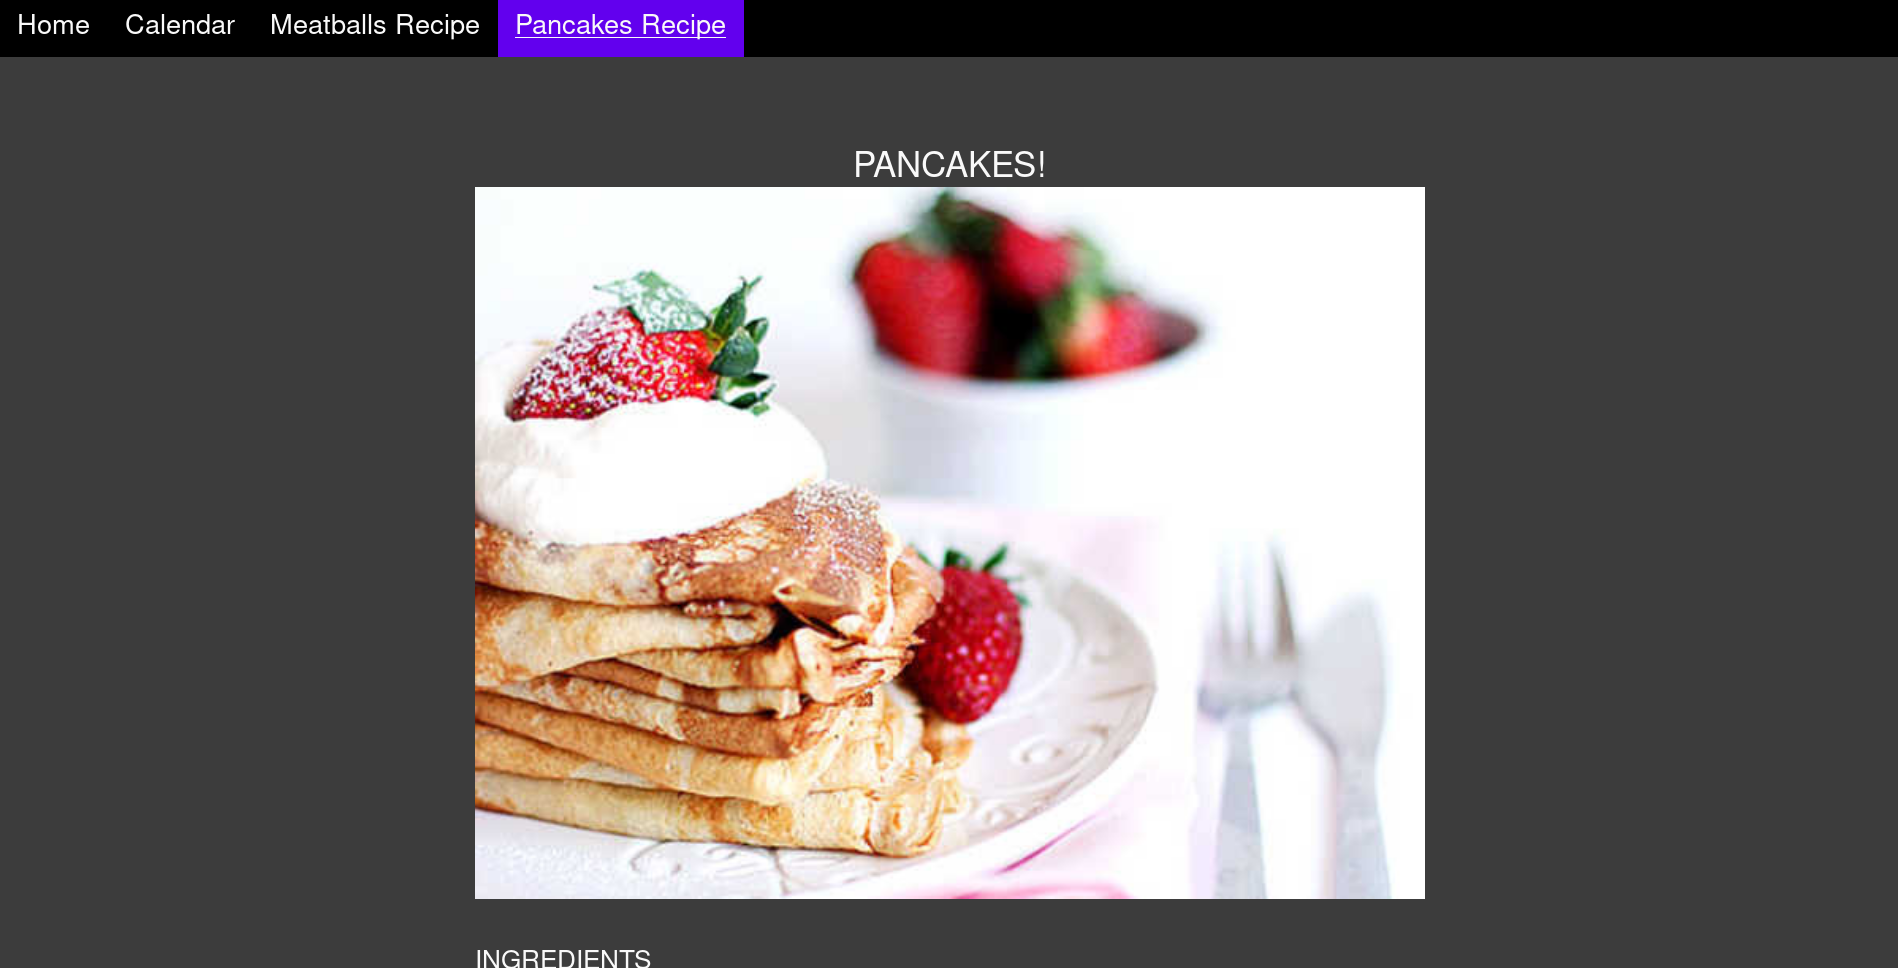
\includegraphics[scale=0.2]{images/pancakes-picture.png}
        \caption{A sample user interface screenshot to illustrate the top of the pancake recipe page.}
        \label{fig:pancakes-picture}
    \end{center}
\end{figure}

\begin{figure}[h!]
    \begin{center}
        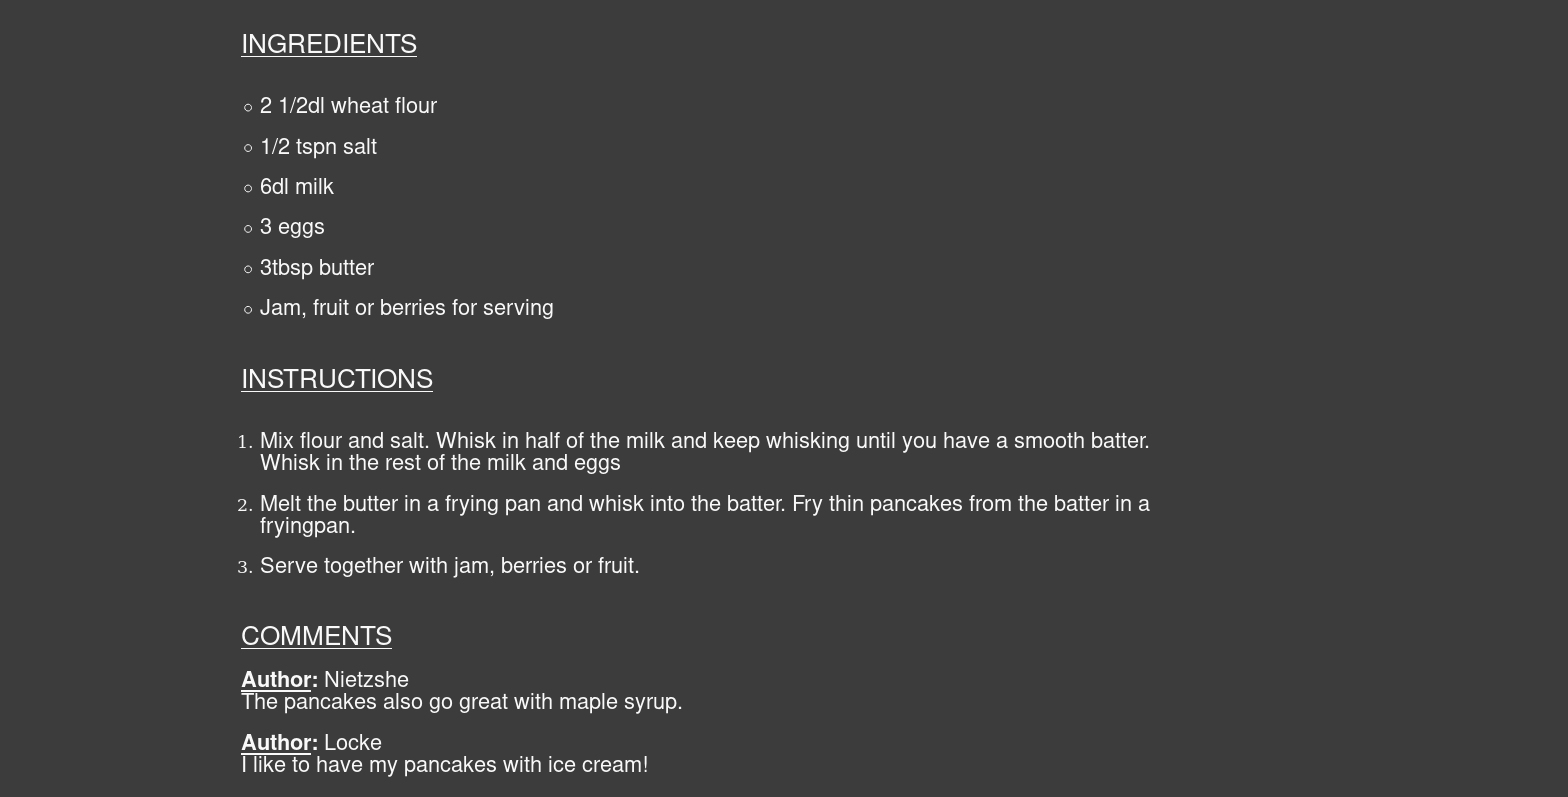
\includegraphics[scale=0.2]{images/pancake-text.png}
        \caption{A sample user interface screenshot to illustrate the bottom of the pancake recipe page.}
        \label{fig:pancake-text}
    \end{center}
\end{figure}

\begin{figure}[h!]
    \begin{center}
        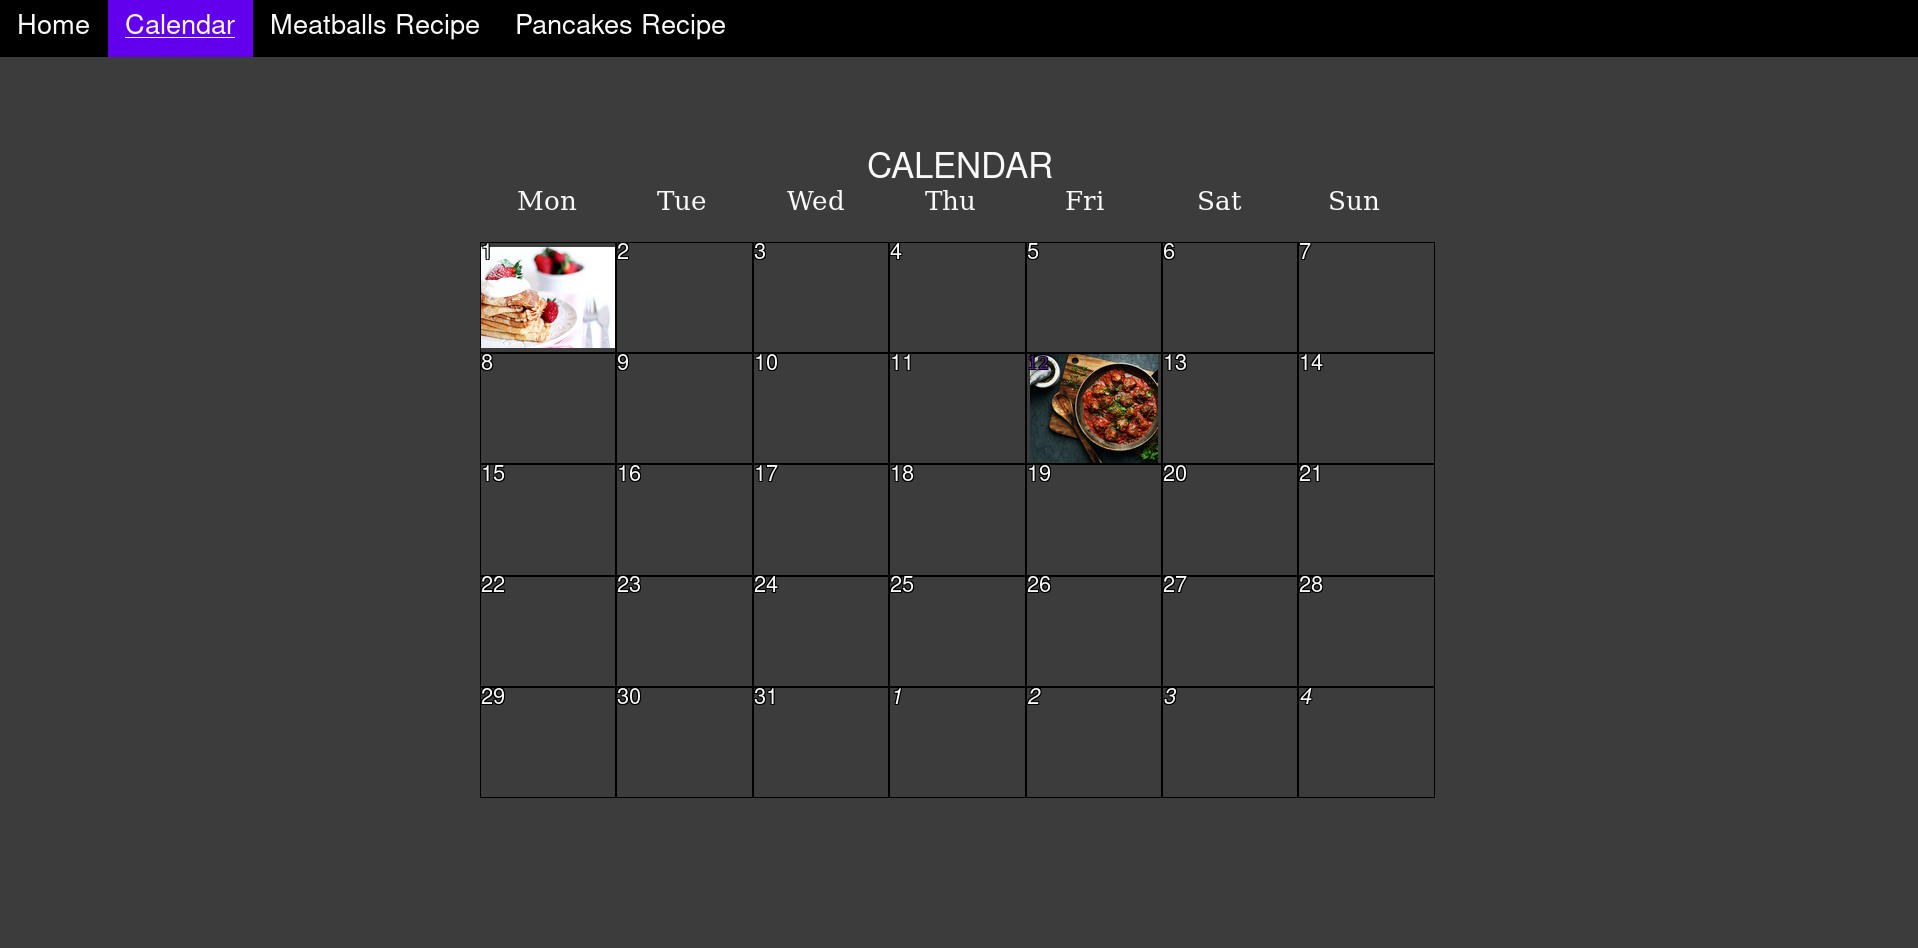
\includegraphics[scale=0.2]{images/calendar.png}
        \caption{A sample user interface screenshot to illustrate the calendar page.}
        \label{fig:calendar}
    \end{center}
\end{figure}

To validate the HTML and CSS files the W3 validators \citet{noauthor_w3c_nodate} and \citet{noauthor_w3c_nodate-1} were used. The results are shown in figures \ref{fig:index-validated}-\ref{fig:mystyles-validated}.

\begin{figure}[h!]
    \begin{center}
        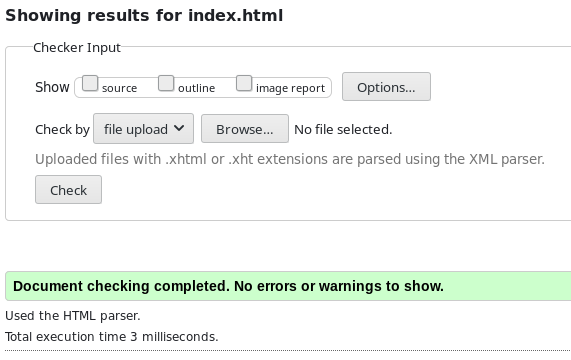
\includegraphics[scale=0.2]{images/index-validated.png}
        \caption{A screenshot showing the index page passing validation.}
        \label{fig:index-validated}
    \end{center}
\end{figure}

\begin{figure}[h!]
    \begin{center}
        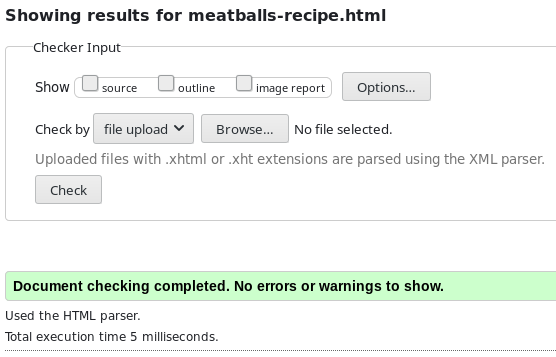
\includegraphics[scale=0.2]{images/meatballs-validated.png}
        \caption{A screenshot showing the meatballs page passing validation.}
        \label{fig:meatballs-validated}
    \end{center}
\end{figure}

\begin{figure}[h!]
    \begin{center}
        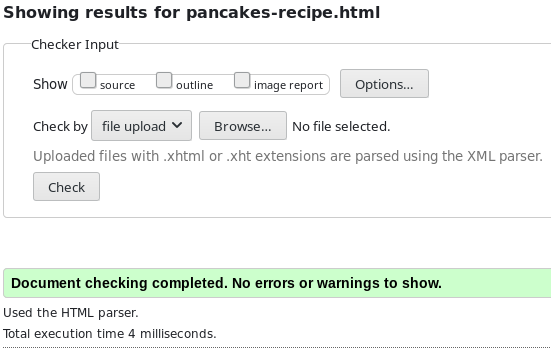
\includegraphics[scale=0.2]{images/pancakes-validated.png}
        \caption{A screenshot showing the pancakes page passing validation.}
        \label{fig:pancakes-validated}
    \end{center}
\end{figure}

\begin{figure}[h!]
    \begin{center}
        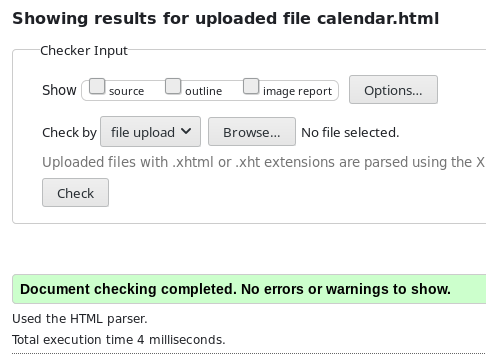
\includegraphics[scale=0.2]{images/calendar-validated.png}
        \caption{A screenshot showing the calendar page passing validation.}
        \label{fig:calendar-validated}
    \end{center}
\end{figure}

\begin{figure}[h!]
    \begin{center}
        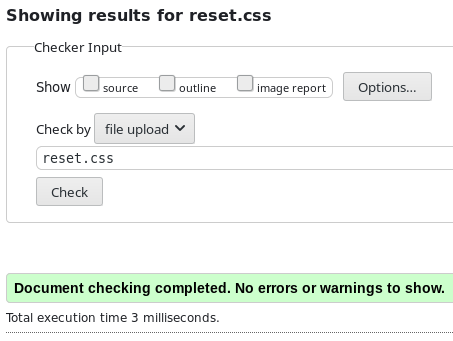
\includegraphics[scale=0.2]{images/reset-validated.png}
        \caption{A screenshot showing the reset CSS passing validation.}
        \label{fig:reset-validated}
    \end{center}
\end{figure}

\begin{figure}[h!]
    \begin{center}
        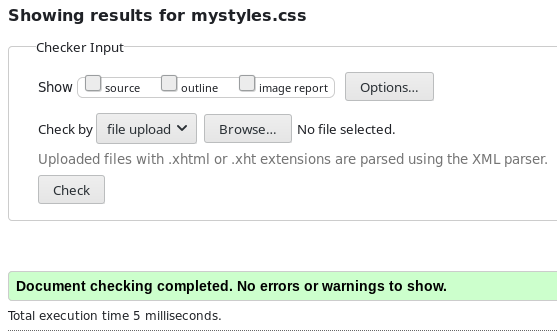
\includegraphics[scale=0.2]{images/mystyles-validated.png}
        \caption{A screenshot showing the mystyles CSS passing validation.}
        \label{fig:mystyles-validated}
    \end{center}
\end{figure}

The first heuristic which concerns the visibility of the system status has been taken into consideration when designing the navigation bar. To infor the user about what is going on the current page that is being visited is being colored in a different color in the navigation bar. In addition it is also underlined. This can be seen in figure \ref{fig:navbar}. The second heuristics is taken into consideration when chosing names for the different pages in the navbar. Names that can easily be understood by the user by not being technical have been chosen which also can be seen in figure \ref{fig:navbar}. In addition, the ingredients for the recipes are presented in a bullet list, and the instructions are presented in a numbered bullet list. Both of these should be very intuitive to the user and require no further explaining. These can be seen in figure \ref{fig:pancake-text}. The consitency and standards heuristic has been put into consideration when navigating between different pages. Instead of learning new ways of navigation a very common navigation bar has been put at the top of the page easily available for the user. When designing the navbar the sixth heuristics has been taken into consideration such that the user can easily recognise how the navbar is used rather than try to recall some complicated instructions from memory. This is done by highlighting the current page and also highlighting when the mouse hovers over a different page as to show that the user is about to commit to a page switch if they press that specific button. The minimalistic and aesthetic design has been put into consideration when choosing the colors for the page and when displaying information. To no reinvent the wheel, aesthetic colors have been chosen from the Material Design framework \citet{noauthor_design_nodate}. A minimalistic design has been presented by not overwhelming the user with information. A single navbar is used to navigate the entirity of the website and all the necessary information is gathered under a single page instead of splitting it up into several. The flow of the individual pages follow a very intuitive pattern.

As the tools suggested for testing the website in different browser (browshershots.org and turbo.net) doesnt allow for testing of local versions of websites (not even using localhost), the author was unable to test the website for other browsers than chrome and firefox, being that these two are the only ones who run natively on GNU/Linux. However, figure \ref{fig:chrome} shows the calendar page running in chrome. The calendar page was chosen as demonstration as it contains much the same formatting as the other pages and more. We can see from the screenshot that the webpage is displayed precisely the same way as the previous screenshot which was taken in firefox making it such that the requirement is met.

\begin{figure}[h!]
    \begin{center}
        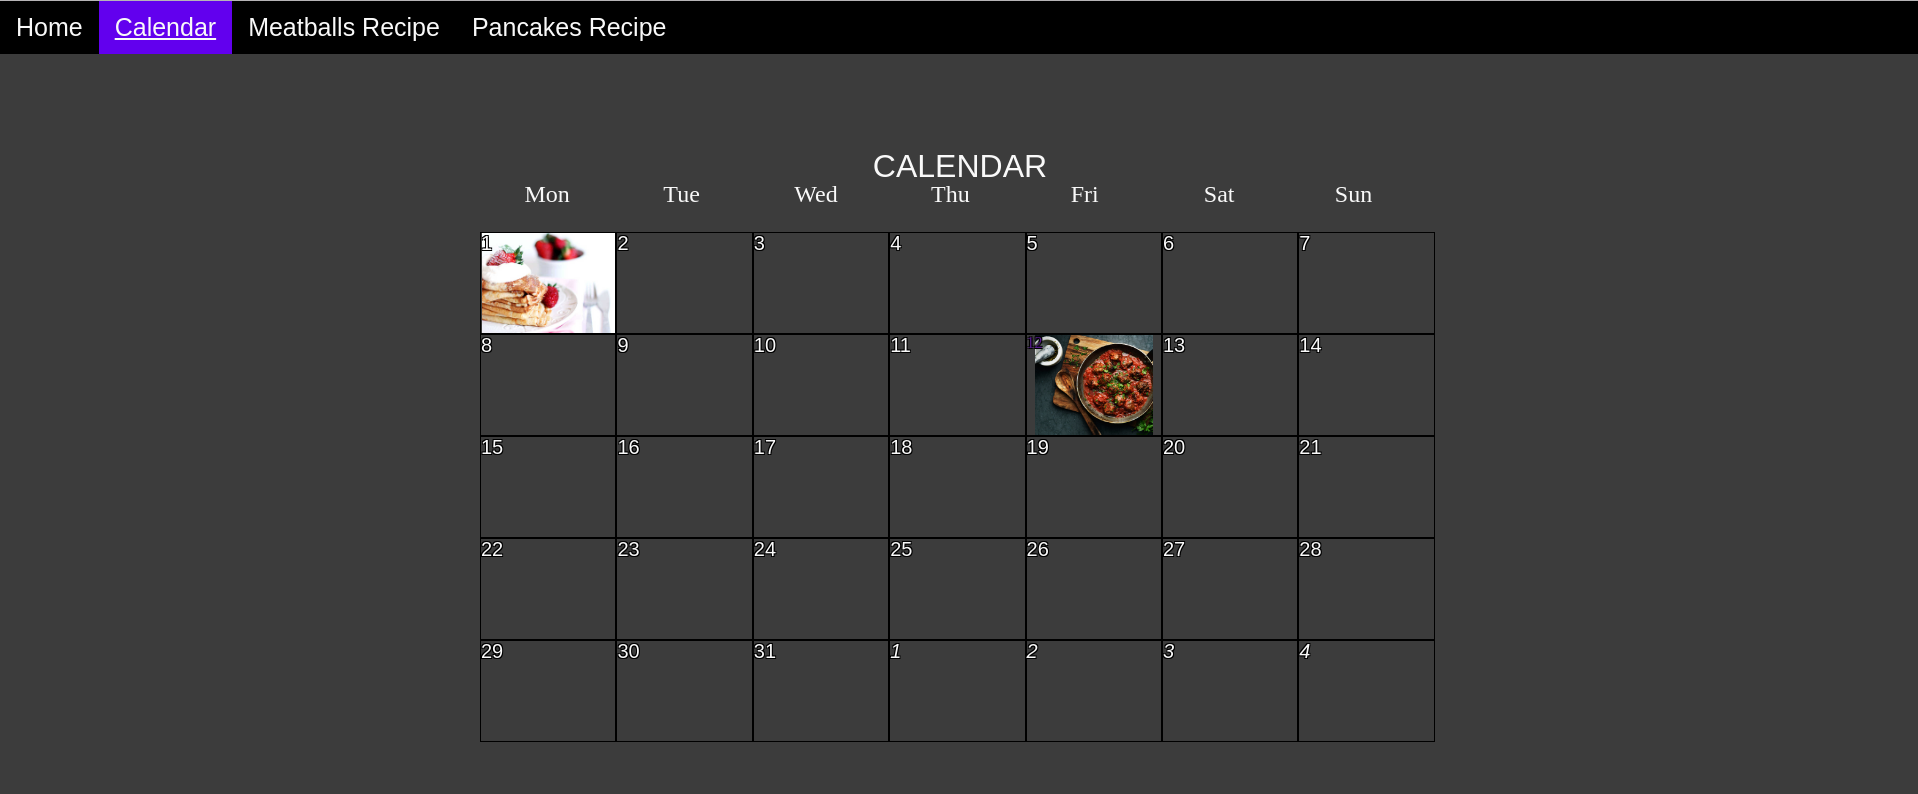
\includegraphics[scale=0.2]{images/chrome.png}
        \caption{A sample user interface screenshot to illustrate the calendar page running in chrome.}
        \label{fig:chrome}
    \end{center}
\end{figure}

\section{Discussion}

Here follows a summary of all of the requirements formated as a bullet list and a check next to each requirement that has been shown to be met earlier in the report.
\begin{itemize}
    \item Design and functionality. \checkmark
    \item Index page. \checkmark
    \item Recipe pages. \checkmark
    \item Calendar page. \checkmark
    \item Tasks. \checkmark
    \begin {itemize}
        \item Pass W3 validations. \checkmark
        \item Use a reset sheet. \checkmark
        \item Use interface design heuristics. \checkmark
        \item Identical behaviour in different browsers. \checkmark
    \end{itemize}

\end{itemize}

The most valuable lesson has been how to use CSS to format HTML divs into a grid network of desired look. This is valuable as the knowledge can be extended to format whole webpages using divs and not just something as specific as calenders. The problem that took the longest was getting borders around the individual dates in the calendar. A problem that was shown to be caused by faulty property
\noindent Summarize the requirements and \textit{clearly state which of them you have met}. What lessons have you learned and what problems did you face? How were the problems solved? Should you have done something differently?

\section{Comments About the Course}

The author has probably spent around 20 hours on this assignment. Worth noting is that the author did not attend any of the first three lectures. Other thoughts is that the assignment is a very good challenge to get started and understand the interplay between HTML and CSS and makes the student look forward to the next assignment. Unfortunately the student came into the course late, which also was the reason for missing the first three lectures. The student thinks it would be interesting to see how the assignment would play out after attending the lectures as less time would probably have to be spen on getting started with the essentials.

\printbibliography

\end{document}
